\documentclass[a4paper, 11pt]{article}
\usepackage{amsmath}
\usepackage{amsfonts}
\usepackage{amssymb}
\usepackage{amsthm}
\usepackage{caratula}
\usepackage{listings}
\usepackage[utf8]{inputenc}
\usepackage[spanish, activeacute]{babel}
\usepackage[usenames,dvipsnames]{color}
\usepackage[width=15.5cm, left=3cm, top=2.5cm, height= 24.5cm]{geometry}
\usepackage{graphicx}
%\usepackage{subcaption}
\usepackage[all]{xy}
\usepackage{multicol}
\usepackage{subfig}
\usepackage{algorithm}
\usepackage{algorithmic}
\usepackage{cancel}
\usepackage{float}
\usepackage{xcolor}
\usepackage{color,hyperref}
\setcounter{secnumdepth}{3} %%agrego subsubsection

\newtheorem{lema}{Lema}
\newtheorem{teorema}{Teorema}
\newtheorem{corolario}{Corolario}
\newtheorem*{correctidud}{Correctitud del algoritmo}
\newtheorem*{notacion}{Notación}

\lstset{breaklines=true, breakatwhitespace=true}
\lstset{numbers=left, numberstyle=\scriptsize}
\lstset{
     literate=%
         {á}{{\'a}}1
         {í}{{\'i}}1
         {é}{{\'e}}1
         {ý}{{\'y}}1
         {ú}{{\'u}}1
         {ó}{{\'o}}1
         {ě}{{\v{e}}}1
         {š}{{\v{s}}}1
         {č}{{\v{c}}}1
         {ř}{{\v{r}}}1
         {ž}{{\v{z}}}1
         {ď}{{\v{d}}}1
         {ť}{{\v{t}}}1
         {ñ}{{\~n}}1                
         {ů}{{\r{u}}}1
         {Á}{{\'A}}1
         {Í}{{\'I}}1
         {É}{{\'E}}1
         {Ý}{{\'Y}}1
         {Ú}{{\'U}}1
         {Ó}{{\'O}}1
         {Ě}{{\v{E}}}1
         {Š}{{\v{S}}}1
         {Č}{{\v{C}}}1
         {Ř}{{\v{R}}}1
         {Ž}{{\v{Z}}}1
         {Ď}{{\v{D}}}1
         {Ť}{{\v{T}}}1
         {Ň}{{\v{N}}}1                
         {Ů}{{\r{U}}}1    
}


%%%%%%%%%%%%%% ALGUNAS MACROS %%%%%%%%%%%%%%
% For \url{SOME_URL}, links SOME_URL to the url SOME_URL
\providecommand*\url[1]{\href{#1}{#1}}

\setlength{\parskip}{10pt plus 1pt minus 1pt}
\usepackage{tikz}
\def\checkmark{\tikz\fill[scale=0.4](0,.35) -- (.25,0) -- (1,.7) -- (.25,.15) -- cycle;}

% Same as above, but pretty-prints SOME_URL in teletype fixed-width font
\renewcommand*\url[1]{\href{#1}{\texttt{#1}}}

% Comando para poner el simbolo de Reales
\newcommand{\real}{\hbox{\bf R}}

\providecommand*\code[1]{\texttt{#1}}

%uso: \ponerGrafico{file}{caption}{scale}{label}
\newcommand{\ponerGrafico}[4]
{\begin{figure}[H]
	\centering
	\subfloat{\includegraphics[scale=#3]{#1}}
	\caption{#2} \label{fig:#4}
\end{figure}
}

\renewcommand{\algorithmiccomment}[1]{\hfill #1}

%%%%%%%%%%%%%%%%%%%%%%%%%%%%%%%%%%%%%%%%%%%%

\materia{Algoritmos y Estructuras de Datos III}

\titulo{Trabajo práctico 2}
%\fecha{fecha de entrega}
%\grupo{Nro grupo}
\integrante{Sebastián Fernandez Ledesma}{392/06}{sfernandezledesma@gmail.com}
\integrante{Fernando Gasperi Jabalera}{56/09}{fgasperijabalera@gmail.com}
\integrante{Maximiliano Wortman}{892/10}{maxifwortman@gmail.com}
\integrante{Santiago Camacho}{110/09}{santicamacho90@gmail.com}


\include{templates}

\begin{document}
\pagestyle{myheadings}
\maketitle
%\markboth{Nombre materia}{Nombre TP}

\thispagestyle{empty}
\tableofcontents

%\setcounter{section}{-1}

\newpage
\section{Problema 1: Plan de vuelo}

\subsection{Presentación del problema}

Se quiere crear un sitio web para reservas de pasajes de avi\'on. El sitio debe tener un sistema de b\'usqueda de itinerarios de vuelo. Un itinerario de vuelo, es una sucesi\'on de vuelos los cuales logran llevarte hacia un destino. Dado una ciudad de salida, y una ciudad de llegada, se busca crear un itinirario de vuelos que me lleve desde la ciudad de salida hasta la de llegada.

Dentro de este itinerario, cada vuelo tiene un horario de despegue y uno de aterrizaje. 

Para poder ser un itinerario valido, la ciudad de destino de un vuelo, tiene que ser la ciudad de llegada del pr\'oximo o directamente el destino donde queriamos llegar, y en particular cada vez que llego a una ciudad debo esperar al menos dos horas desde el aterrizaje, para poder tomarme un vuelo, lo cual resulta l\'ogico dado que una persona puede necesitar al menos ese tiempo para tr\'amites de aeropuerto.

Es por eso que se nos pide el mejor itinerario, teniendo al menos dos horas entre cada vuelo, donde mejor itinerario es el que primero llega a la ciudad destino.

Adem\'as se nos pide que la resoluci\'on de este problema se implemente en un complejidad no peor a O($N^{2}$) donde N es la cantidad de vuelos totales que existen en todo el sistema (formen parte del itinerario o no).
\subsection{Resolución}

Sea Ciudad un renombre de String.

Sea Vuelo una tupla $<$despegue:Nat, aterrizaje:Nat, origen:Ciudad, destino:Ciudad$>$

Dado $vuelos$:Conj(Vuelo):

Llamemos a $ciudadades$:Conj(Ciudad) al conjunto tal que:

($\forall$ $c$:Ciudad, $c$ $\in$ $ciudades$)  $\Leftrightarrow$ ($\exists$ $v$:Vuelo, $v$ $\in$ $vuelos$ $\wedge$ ($v$.origen $\equiv$ $c$ $\vee$ $v$.destino $\equiv$ $c$))

Dadas $a,b$:Ciudad, $a,b \in ciudades$. 

Sea el enunciado:

esItinerarioValido(Sec$<$Vuelo$>$ $S$, Ciudad a, Ciudad b) $\equiv$

 
$S_{0}$.origen $\equiv a \wedge S_{S.tamanio-1)}$.destino$ \equiv b \wedge$ 

($\forall$ $i$:Nat, 0 $<$ i $<S.tamanio$)($S_{i}$.destino $\equiv$ $S_{i+1}$.origen $\wedge$ $S_{i}$.aterrizaje + 2 $\leq$ $S_{i+1}$.despegue))

Se nos pide encontrar $S$:Sec$<$Vuelo$>$ tal que 

esItinerarioValido($S$,a,b) $\wedge$ 

$(\forall$ $S'$:Sec$<$Vuelo$>$ $/$ esItinerarioValido($S'$,a,b) $\implies$  

$S_{S.tamanio-1}$.aterrizaje$) \leq S'_{S'.tamanio-1}$.aterrizaje))

\subsection{Demostración}

\subsection{Análisis de complejidad}

\subsection{Tests de complejidad}


\newpage
\section{Problema 2: Caballos salvajes}

\subsection{Presentación del problema}
En este problema nos presentan un tablero de dimensiones conocidas pero no acotadas
del mismo tipo que el de ajedrez, es decir un tablero cuadriculado y cuadrado:\\
\begin{figure}[H]
	\begin{minipage}[t]{\linewidth}
		\centering
		
\includegraphics[scale=0.5]{show_dimension.png}
		%\caption{}
		\label{fig:p2_complejidad_varia_k}
	\end{minipage}
\end{figure}
y un conjunto de caballos, piezas de ajedrez, en casillas también conocidas, por ejemplo:\\
\begin{figure}[H]
	\begin{minipage}[t]{\linewidth}
		\centering
		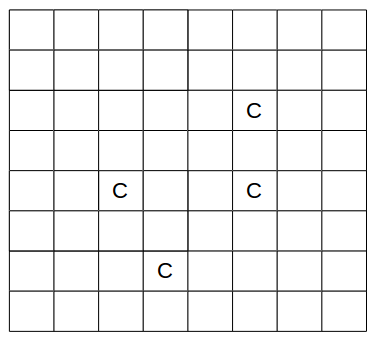
\includegraphics[scale=0.5]{show_horses.png}
		%\caption{}
		\label{fig:p2_complejidad_varia_k}
	\end{minipage}
\end{figure}
el objetivo es reunir a todos los caballos en una misma casilla del tablero con una cantidad
de movimientos total, es decir sumando los movimientos que le tomo a cada uno de los caballos, mínima.
Los movimientos permitidos a los caballos son los mismos que los impuestos por las reglas de ajedrez:\\
\begin{figure}[H]
	\begin{minipage}[t]{\linewidth}
		\centering
		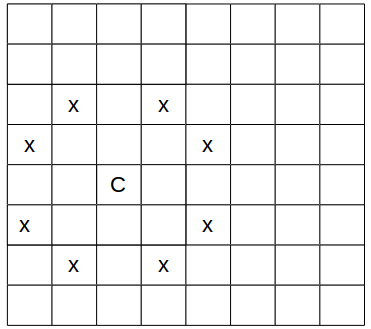
\includegraphics[scale=0.5]{show_jumps.png}
		\caption{La C representa la casilla donde está ubicado el caballo y X los lugares a los cuales podría saltar.
}
		\label{fig:p2_complejidad_varia_k}
	\end{minipage}
\end{figure}
A continuación mostramos un tablero de $4 \times 4$ en el cual los caballos comienzan en las esquinas, donde
aparecen las C pequeñas. Los números dentro de las casillas representan la suma de las distancias de los caminos
mínimos de cada uno de los caballos hasta esa casilla. Por ejemplo, la casilla correspondiente a la fila 2 y
columna 4 (contando las filas desde abajo para arriba y las columnas de izquierda a derecha comenzando ambas desde 1)
tiene el número 2 porque los dos caballos pueden llegar a ella en sólo 1 movimiento. Por lo tanto la suma en este
caso es $1 +1 = 2$. Las casillas que están coloreadas se corresponden con las posibles soluciones de la instancia,
son todas mínimas.
\begin{figure}[H]
	\begin{minipage}[t]{\linewidth}
		\centering
		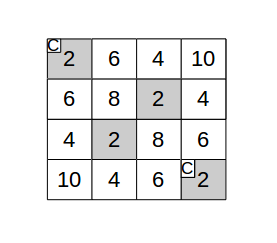
\includegraphics[scale=0.5]{show_solution.png}
		\label{fig:p2_complejidad_varia_k}
	\end{minipage}
\end{figure}

\subsection{Resolución}
Nosotros modelamos el problema con grafos con lo cual resultó equivalente al de camino mínimo 
con un origen y múltiples destinos en un grafo no dirigido sin peso en las aristas. 
En este caso en particular las aristas no tienen peso porque el salto de un caballo siempre 
tiene el mismo costo. En un grafo con las características mencionadas el algoritmo de 
Breadth First Search \cite[p.~522]{cormen} obtiene el camino mínimo entre el origen tomado y el resto de los nodos,
éste es el camino entre el origen y el nodo en árbol generado.
El modelo consiste en tomar a las casillas del tablero como nodos del grafo, las casillas en las que 
hay caballos como nodos origen y existe una arista entre dos nodos, casillas, si de una a la otra se
puede ir con un salto de caballo. Cabe destacar que el salto de caballo es simétrico: si con un salto
de caballo se puede ir de la casilla $a$ a la $b$ entonces necesariamente también se puede con un 
salto de caballo ir de la casilla $b$ a la $a$:\\
\begin{figure}[H]
	\begin{minipage}[t]{0.5\linewidth}
		\centering
		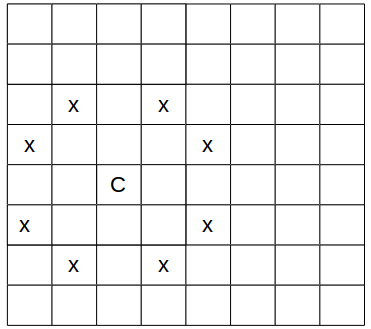
\includegraphics[scale=0.5]{show_jumps.png}
		\label{fig:p2_complejidad_varia_k}
	\end{minipage}
	\begin{minipage}[t]{0.5\linewidth}
		\centering
		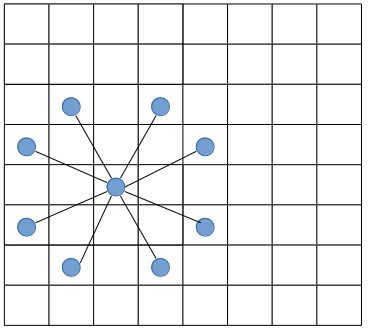
\includegraphics[scale=0.5]{show_graph.png}
		\label{fig:p2_complejidad_varia_k}
	\end{minipage}
\end{figure}
Los pasos para resolver el problema una vez modelado son bastante directos:
\begin{enumerate}
  \item Recorrer el grafo una vez por cada caballo presente tomando como origen el nodo, casilla, en la 
    que se encuentra el caballo.
  \item Guardar, en cada nodo, la cantidad de saltos que le toma a cada caballo llegar a él.
  \item Recorrer todos los nodos y quedarse con alguno de los de suma mínima.
\end{enumerate}
Hay un conjunto pequeño de instancias para los cuales la solución del problema es trivial:
\begin{description}
  \item[$n = 1$] los caballos sólo pueden estar en una casilla por lo cual la solución es la única casilla
    que existe y la cantidad de movimientos totales es 0.
  \item[$n = 2$] los caballos no pueden realizar movimiento permitido alguno. Sólo existe solución en el caso
    en el que los caballos se encuentran todos en la misma casilla.
  \item[$n = 3$] existe solución siempre excepto cuando un caballo comienza en la casilla central del tablero
    en cuyo caso no tiene movimientos permitidos y del resto de las casillas no existe forma de llegar a la
    casilla central mediante movimientos permitidos, lo cual es trivial si vemos que desde la casilla central
    no existen movimientos permitidos porque como ya mencionamos los movimientos del caballo son simétricos.
  \item[$n > 4$] se puede probar fácilmente que de cualquier casilla del tablero se puede acceder a cualquier otra,
    por lo tanto cuando la dimensión del tablero es mayor a 4 siempre existe solución.
\end{description}
En el pseudocódigo no mostramos el manejo de instancias que poseen un tablero de dimensión menor a 4 porque
al ser muy particulares no aportan mayor claridad a la presentación de la idea central del algoritmo.

\subsection{Pseudocódigo}
\begin{algorithm}[H]
  \begin{algorithmic}
    %\STATE $\gets$ \WHILE{} \ENDWHILE \IF{} \ELSE \ENDIF
    \STATE $distancias$ $\gets$ Matriz($n$, $n$)
    \STATE $tablero$ $\gets$ Tablero($n$, $n$)
    \STATE $caballos$ $\gets$ Conj($Casilla$)
    \WHILE {$caballos \neq \emptyset$}
      \STATE $origen$ $\gets$ $caballos$.next()
      \STATE BFS($origen$, $tablero$, $distancias$)
    \ENDWHILE
    \STATE ($suma_{min}$, $casilla_{min}$) $\gets$ MIN($distancias$)
    \caption{caballos\_salvajes}
  \end{algorithmic}
\end{algorithm}

\begin{algorithm}[H]
  \begin{algorithmic}
    %\STATE $\gets$ \WHILE{} \ENDWHILE \IF{} \ELSE \ENDIF
    \STATE $nodos_{no visitados}$ $\gets$ Cola
    \STATE push($nodos_{no visitados}$, $origen$)
    \STATE $tablero_{origen}$ $\gets$ 0
    \STATE $vecinos$ $\gets$ Cola
    \WHILE {$nodos_{no visitados} \neq \emptyset$}
      \STATE $nodo_{actual}$ $\gets$ pop($nodos_{no visitados}$)
      \STATE $vecinos$ $\gets$ obtener\_vecinos($nodo_{actual}$)
      \WHILE {$vecinos \neq \emptyset$}
        \STATE $vecino$ $\gets$ pop($vecinos$)
        \IF {$neg$ esta\_marcado($tablero$, $vecino$)}
          \STATE $tablero_{vecino}$ $\gets$ $tablero_{nodo_{actual}}$+1
          \STATE $distancias_{vecino}$ $\gets$ $distancias_{vecino}$ + $tablero_{vecino}$
          \STATE push($nodos_{no visitados}$, $vecino$)
        \ENDIF
      \ENDWHILE
    \ENDWHILE
    \caption{BFS}
  \end{algorithmic}
\end{algorithm}

\subsection{Demostración de correctitud}
Una instancia del problema está dada por la dimensión del tablero $n$ y la posición
de los $k$ caballos. Luego de modelarlo tenemos un grafo $G = (V, E)$ tal que $\left\vert{V}\right\vert = n^2$, uno
por cada nodo, y $\left\vert{E}\right\vert < n^2 * 4$. La cota superior sobre las aristas proviene del hecho de que
un caballo sólo pude saltar a 8 casillas diferentes como máximo, asumiendo que todos los
saltos posibles caen dentro del tablero. Por lo tanto, la cantidad de aristas debe ser menor
a $\frac{n^2 * 8}{2}$ porque en muchas casillas, como las de las esquinas o las de las bandas, la
mayoría de los saltos posibles caen fuera del tablero. Los caballos los representaremos con un multiconjunto
de nodos al que llamaremos $origenes$, $\left\vert{origenes}\right\vert = \left\vert{caballos}\right\vert = k$. Utilizamos un multiconjunto 
para representarlos porque inicialmente puede haber más de un caballo en una casilla determinada.
Sea $PS_{v,u}$ el conjunto de los caminos posibles entre el nodo $u$ y el nodo $v$.
Dado un nodo $v$ el conjunto de soluciones posibles asociado a $v$ es $SP_v$:
\begin{displaymath}
  SP_v = \left\{ { \sum_{u \in origenes} \left\vert{P_{u,v}}\right\vert : P_{u, v} \in PS_{u, v}} \right\}
\end{displaymath}
La solución óptima para un nodo $v$ la denominaremos $SP_v^{opt}$ y está determinada de la siguiente forma:
\begin{displaymath}
  SP_v^{opt} = \min \left\{ {s : s \in SP_v} \right\} 
\end{displaymath}

\begin{lema}
\label{lema_p2}
Una solución óptima para un nodo $v$ está compuesta por caminos mínimos entre los orígenes
y $v$:
\begin{displaymath}
  s = SP_v^{opt} \Leftrightarrow s = \sum_{u \in origenes} \min \left\{ { \left\vert{P}\right\vert : P \in PS_{u, v}} \right\}
\end{displaymath}
\end{lema}
\begin{proof}
  Sea $SP_{opt}$ una solución óptima para el nodo $v$ que contiene un camino $P_{w,v}$ no mínimo. Sea $P_{w,v}^{min}$ 
un camino mínimo entre $w \in origenes$ y $v$. Sea $SP'_{opt}$:
\begin{displaymath}
SP'_{opt} = SP_{opt} \setminus P_{w, v} \cup \left\{{P_{w,v}^{min}}\right\}
\end{displaymath}
veamos el costo de $SP'_{opt}$ expresado en función del de $SP_{opt}$:
\begin{displaymath}
  SP'_{opt} = \sum_{u \in origenes} \left\vert{P_{u,v}}\right\vert - \left\vert{P_{w,v}}\right\vert + \left\vert{P_{w,v}}\right\vert
\end{displaymath}
pero dado que $P_{w,v}$ no es mínimo:
\begin{displaymath}
  P_{w,v} > P_{w,v}^{min} \Rightarrow P_{w,v} - P_{w,v}^{min} > 0
\end{displaymath}
pero entonces volviendo a la ecuación anterior nos queda que:
\begin{displaymath}
  SP'_{opt} < SP_{opt}
\end{displaymath}
Lo cual es absurdo porque partimos suponiendo que $SP_{opt}$ era un solución óptima y por lo tanto mínima.
\end{proof}

Finalmente, caracterizaremos a la solución del problema $S$:
\begin{displaymath}
  S = \min_{v \in V} \left\{ {SP_{v}^{opt}} \right\}
\end{displaymath}
Nuestro algoritmo calcula el peso del camino mínimo entre cada uno de los orígenes y el resto de los nodos \cite[p.~522]{cormen} 
Luego suma en cada nodo $v$ el peso de los caminos mínimos desde cada uno de los orígenes hasta él que por \textbf{Lema 1} es
igual a $SP_{v}^{opt}$. Por último, recorre todos los nodos y toma el mínimo entre todos los $SP_{v}^{opt}$ calculados
lo cual es precisamente la solución que acabamos de definir.

\subsection{Análisis de complejidad}
El algoritmo tiene 3 partes importantes a considerar con respecto a su complejidad:
\begin{enumerate}
  \item generar el grafo que modela la instancia del problema
  \item aplicar BFS una vez por cada caballo con el nodo correspondiente al caballo como origen
  \item buscar el nodo que cuente con la suma mínima
\end{enumerate}
Generar el grafo que modela la instancia del problema recibida tiene costo $O(\left\vert{V}\right\vert) = O(n^2)$. 
Sólo precisamos una matriz de tamaño $n \times n$. Cada posición representa a un nodo y en él almacenaremos la suma
de los caminos mínimos desde cada uno de los caballos hasta él. No es necesario guardar información acerca de las
aristas del grafo porque, al ser el salto de del caballo un movimiento conocido, dado un nodo se pueden obtener sus vecinos
en tiempo constante $O(1)$ calculándolos \textit{ad hoc}.
Tampoco es necesario guardar la distancia desde cada origen hasta cada uno de los nodos ya que sólo nos interesará
la suma total sobre cada nodo. Por lo tanto, basta con ir sumando la distancia de cada uno de los orígenes hasta él.\\
El costo de aplicar BFS es $O(\left\vert{E}\right\vert + \left\vert{V}\right\vert) = O(n^2 * 8 + n^2) = O(n^2)$ \cite[1]{cormen} porque, 
como ya vimos, la cantidad de aristas del grafo está acotada por la cantidad de nodos, porque el caballo a lo sumo
puede saltar a 8 casillas diferentes.\\
Por último, buscar el mínimo tiene un costo $O(\left\vert{V}\right\vert) = O(n^2)$ porque simplemente consiste
en iterar por todos los nodos y quedarse con el que tenga la suma mínima.\\
Por lo tanto, la complejidad está dada por:
\begin{displaymath}
  O(construir\_grafo) + \#caballos * O(BFS) + O(obtener\_minimo) = 
\end{displaymath}
\begin{displaymath}
  O(n^2) + k * O(n^2) + O(n^2) = O(k * n^2)
\end{displaymath}
La cota obtenida $O(n^2 * k)$ es además válida para $\Theta (n^2 * k)$ porque lo único que puede variar de una
instancia a otra del mismo tamaño es la posición de los caballos en el tablero. Sin embargo, la cantidad de nodos
y aristas del grafo es independiente de la posición de los caballos en el tablero. Por lo tanto, el costo de
construir el grafo, recorrerlo con BFS y luego recorrer todos los nodos para obtener el de suma mínima
es el mismo para todas las instancias del mismo tamaño.

\subsection{Tests de complejidad}
El objetivo de las experimentaciones que realizaremos es corroborar que las cotas obtenidas por nuestro análisis
de complejidad son reflejadas por los resultados empíricos. Como la cota depende de la cantidad de caballos
utilizados y las dimensiones del tablero realizaremos dos experimentos:
\begin{enumerate}
  \item Mantendremos la cantidad de caballos ($k$) constante e incrementaremos la dimensión del tablero ($n$) para
    ver si realmente la relación con el crecimiento de la dimensión del tablero es efectivamente cuadrática.
  \item Mantendremos el la dimensión del tablero ($n$) constante e incrementaremos la cantidad de caballos para
    constatar si la relación con la cantidad de caballos es lineal como calculamos.
\end{enumerate}

En el primer experimento variamos la dimensión del tablero desde 1 hasta 100 con un salto de 1. La posición de los
caballos fue elegida pseudo-aleatoriamente, sin restringir que dos caballos tengan la misma posición original.
Para cada dimensión $n$ generamos 10 posicionamientos distintos de los caballos, cada posicionamiento lo ejecutamos
10 veces y nos quedamos con la corrida de menor tiempo de cada posicionamiento para finalmente tomar el promedio
sobre los mínimos de los 10 posicionamientos distintos. Ésto lo realizamos para $k = 5, 10, 15$. El gráfico
que muestra los resultados es el siguiente:
\begin{figure}[H]
	\begin{minipage}[t]{\linewidth}
		\centering
		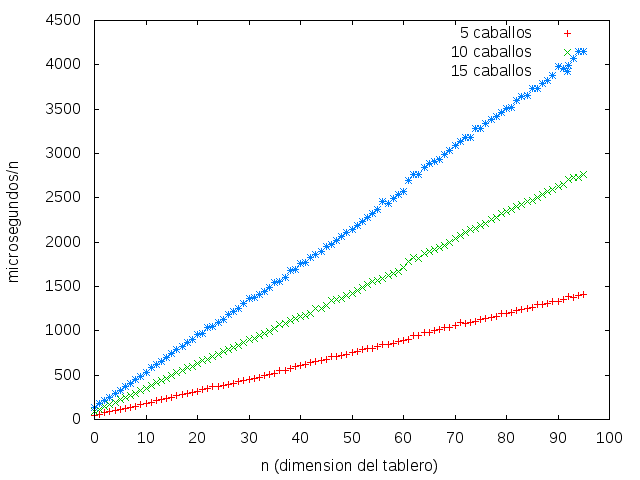
\includegraphics[width=\textwidth]{p2_varia_dimension.png}
		%\caption{}
		\label{fig:p2_complejidad_varia_dimension_tablero}
	\end{minipage}
\end{figure}
Como se ve en el gráfico la cantidad de microsegundos la dividimos por la dimensión del tablero ($n$) y las
curvas resultantes para los 3 casos de caballos se acercan mucho a una recta.

El segundo experimento consistió en tomar un tablero de dimensión fija, en este caso en particular elegimos $n = 40, 70, 100$, y 
variar la cantidad de caballos desde 2 a 50. La posición de los caballos en este caso también fue elegida pseudo-aleatoriamente
y para cada instancia de k caballos la corrimos con 10 posicionamientos distintos de los cuales tomamos el promedio y cada posicionamiento
lo corrimos también 10 veces y nos quedamos con el mínimo. Presentamos los resultados en el siguiente gráfico:
\begin{figure}[H]
	\begin{minipage}[t]{\linewidth}
		\centering
		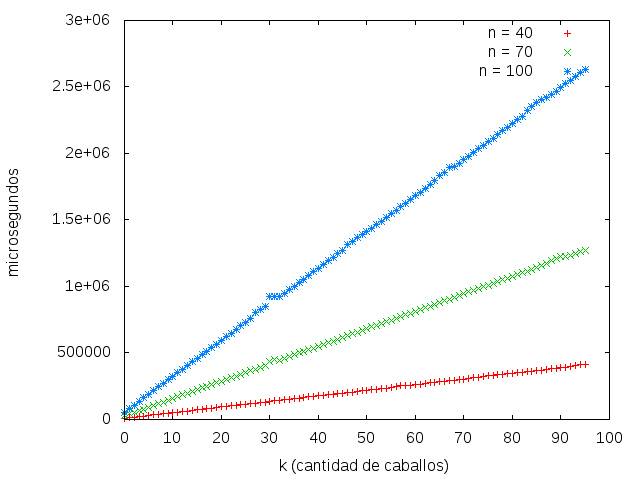
\includegraphics[width=\textwidth]{p2_varia_k.png}
		%\caption{}
		\label{fig:p2_complejidad_varia_k}
	\end{minipage}
\end{figure}



\newpage
\section{Problema 3: La comunidad del anillo}

\subsection{Presentación del problema}

Dado un conjunto de computadoras, y un conjunto de enlaces entre pares de ellas (con a lo sumo un enlace para cada par), los cuales tienen un costo asociado, se pide elegir un conjunto de ellos tales que haya una red en forma ``anillo'', y que todas las computadoras tengan acceso a éste anillo usando enlaces de manera directa o indirecta (es decir, no es necesario que tengan un enlace a una computadora del anillo, sino que pueden tenerlo con una computadora intermedia), de manera de minimizar el costo total de los enlaces elegidos. Veamos por ejemplo las siguientes dos figuras:

\begin{figure}[ht]
	\begin{minipage}[t]{0.5\linewidth}
		\centering
		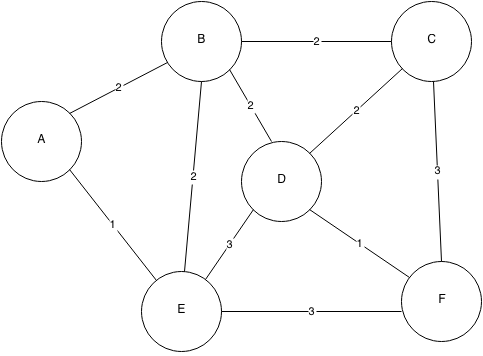
\includegraphics[width=\textwidth]{ej3_ejemplo.png}
		\caption{Red original}
		\label{fig:ej3_ejemplo}
	\end{minipage}
	\begin{minipage}[t]{0.5\linewidth}
		\centering
		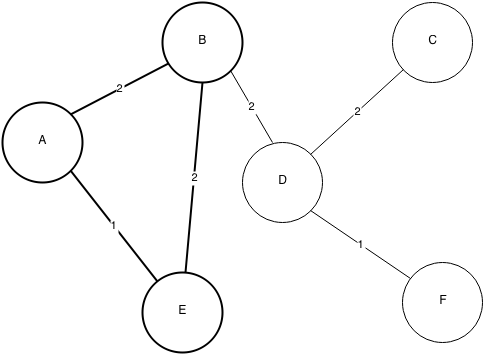
\includegraphics[width=\textwidth]{ej3_ejemplo_solucion_optima.png}
		\caption{Una solución óptima}
		\label{fig:ej3_ejemplo_solucion_optima}
	\end{minipage}
\end{figure}

En la Figura \ref{fig:ej3_ejemplo} vemos una red de seis computadoras con sus enlaces y sus costos asociados, y en la Figura \ref{fig:ej3_ejemplo_solucion_optima} tenemos una solución óptima del problema, con el anillo de equipos remarcado.

\subsection{Resolución}

Primero necesitamos caracterizar al conjunto de soluciones del problema. Como a lo sumo hay un enlace entre dos máquinas, podemos pensar a éstas como vértices, y a los enlaces como aristas. Entonces, tenemos como input un grafo $G = (V,X)$, y una solución (si existe) será un subgrafo de $G$ con las siguientes características:
\begin{enumerate}
    \item Debe ser \textbf{generador}, ya que para toda computadora se cumple que: o forma parte del anillo, o existe un camino simple que lleva a alguna máquina del anillo, y para ésto todas las computadoras deben estar en el subgrafo solución.
    \item Debe ser \textbf{conexo}, porque si no lo fuera, eso implica que hay alguna máquina que no puede conectarse con el anillo.
    \item Debe tener un \textbf{circuito simple}, éste será el anillo. Si no puede contruirse, no habrá solución.
    \item Más aún, debe tener \textbf{exactamente un circuito simple}. El problema no prohíbe que haya más de uno, pero si tuviéramos más de un ciclo, bastaría con quitar la arista más costosa que forme parte de algún circuito para mejorar la solución, ya que el subgrafo seguiría siendo conexo (los caminos simples que pasaran por la arista que quitamos podrían desviarse por el resto del circuito) y seguiría existiendo al menos un circuito simple (si no, este subgrafo sería un árbol, pero entonces agregar la arista que quitamos nos daría un grafo con exactamente un circuito simple, absurdo). Este procedimiento lo podríamos repetir hasta que sólo quede un circuito. Luego, podemos descartar todos los subgrafos con más de un circuito simple, ya que son soluciones necesariamente subóptimas.
\end{enumerate}
Tenemos entonces caracterizada a una solución como un subgrafo generador de $G$ conexo y con exactamente un circuito simple. Una solución óptima entonces será minimizar el costo de este tipo de subgrafos. Vamos a construir una solución óptima en dos pasos:
\begin{enumerate}
 \item Hallaremos $T = (V, X_T)$ un árbol generador mínimo de $G$ (si no existe, no hay solución).
 \item Tomaremos la arista $e$ de mínimo costo en $X - X_T$ (si el conjunto es vacío, no hay solución) y la agregaremos a $T$.
\end{enumerate}
Nuestro algoritmo construirá entonces el subgrafo $S = (V, X_T \cup \left\{e\right\})$. En la demostración de correctitud veremos que efectivamente $S$ es una solución óptima del problema.

Para obtener el árbol generador mínimo usamos el algoritmo de Prim, luego a este grafo le agregaremos la arista más chica de las que no pertenecen a él, y finalmente para encontrar el ciclo usaremos la función $hallarCircuito$, que hace DFS sobre la solución.

\subsubsection{Pseudocódigo}
%aca va el pseudocodigo del problema.
\begin{algorithm}[H]
\begin{algorithmic}[1]
\caption{LaComunidadDelAnillo(aristasGrafo)}
\STATE verticesAGM $\leftarrow$ vacía
\STATE aristasAGM $\leftarrow$ vacía
\STATE aristasCandidatasAGM $\leftarrow$ vacía
\STATE Pongo el vértice 0 en verticesAGM, y sus aristas en aristasCandidatasAGM
\WHILE {$|$aristasAGM$|$ $<$ n - 1 \AND $|$aristasCandidatasAGM$|$ $>$ 0}
	\STATE Tomar la arista candidata de menor costo (quitándola además de las candidatas)
    \IF {La arista incide en dos vértices del AGM}
        \STATE No la puedo usar
    \ELSE
        \STATE Insertar el nuevo vértice en verticesAGM
        \STATE Eliminar la arista de aristasGrafo
        \STATE Insertar la arista en aristasAGM
        \FOR {\textbf{each} arista del nuevo vértice (que no fue considerada antes)}
            \STATE Insertar arista en aristasCandidatasAGM
        \ENDFOR
    \ENDIF
\ENDWHILE
\IF {$|$aristasAGM$|$ $<$ n - 1 \OR $|$aristasGrafo$|$ == 0}
    \STATE No hay solución
\ENDIF
\STATE Arista aristaMenor $\leftarrow$ Arista de menor costo de aristasGrafo
\STATE Vertice primero $\leftarrow$ El primer vértice de aristaMenor (podría ser cualquiera de los dos vértices, no afecta al algoritmo)
\STATE Insertar aristaMenor en aristasAGM
\STATE Defino array de aristas aristaAnterior$[$n$]$
\STATE Defino array de enteros verticeVisitadoCount$[$n$]$ inicializándolo todo en $0$
\STATE Defino array de vertices (enteros) verticeAnterior$[$n$]$ inicializándolo todo en $-1$
\STATE Llamar a la función hallarCircuito(verticeVisitadoCount, primero, verticeAnterior, aristaAnterior)
\end{algorithmic}
\end{algorithm}

Como sabemos que el vértice $primero$ forma parte del circuito simple, las aristas del circuito se pueden obtener pidiendo $aristaAnterior[primero]$, lo que devuelve una arista y un vértice nuevo, al que se le pedirá de nuevo lo mismo, hasta llegar a $primero$.

\begin{algorithm}[H]
\begin{algorithmic}[1]
\caption{Vertice hallarCircuito(verticeVisitadoCount, verticeAnterior, aristaAnterior)}
    \STATE pila$<$Vertice$>$ pilaVertices $\leftarrow$ pila vacía
    \STATE pilaVertices.push(0) \textcolor{CadetBlue}{// Pusheo un vértice para empezar}
    \STATE bool hayCircuito $\leftarrow$ false
    \STATE Vertice res $\leftarrow$ -1
    \WHILE {(\NOT hayCircuito) \AND ($|$pilaVertices$|$ $>$ 0)}
        \STATE Vertice actual $\leftarrow$ pilaVertices.top()
        \STATE pilaVertices.pop()
        \STATE verticeVisitadoCount$[$actual$]$++
        \IF {verticeVisitadoCount$[$actual$]$ == 2}
            \STATE hayCircuito $\leftarrow$ true
            \STATE res $\leftarrow$ actual
        \ELSE
            \FOR {\textbf{each} arista del vértice actual}
                \STATE Vertice nuevoActual $\leftarrow$ El otro vértice de la arista
                \STATE Vertice nuevoAnterior $\leftarrow$ actual
                \IF {nuevoActual == verticeAnterior$[$actual$]$}
                    \STATE \textcolor{CadetBlue}{// Si estoy acá es porque estaba volviendo por la misma arista que vine (formando un circuito NO simple)}
                \ELSE 
                    \STATE aristaAnterior$[$nuevoActual$]$ $\leftarrow$ arista
                    \STATE verticeAnterior$[$nuevoActual$]$ $\leftarrow$ nuevoAnterior
                    \STATE pilaVertices.push(nuevoActual)
                \ENDIF
            \ENDFOR
        \ENDIF
    \ENDWHILE
    \RETURN res
\end{algorithmic}
\end{algorithm}

%\begin{algorithm}[H]
%\begin{algorithmic}[1]
%\caption{hallarCircuito(verticeVisitado, actual, verticeAnterior, aristaAnterior)}
%\IF {\NOT verticeVisitado$[$actual$]$}
    %\STATE verticeVisitado[actual] $\leftarrow$ true
    %\FOR {\textbf{each} arista del vértice actual}
        %\STATE Vertice nuevoActual $\leftarrow$ El otro vértice de la arista
        %\STATE Vertice nuevoAnterior $\leftarrow$ actual
        %\IF {nuevoActual == verticeAnterior$[$actual$]$}
            %\STATE \textcolor{CadetBlue}{// Si estoy acá es porque estaba volviendo por la misma arista que vine (formando un circuito NO simple)}
        %\ELSE
            %\STATE aristaAnterior$[$nuevoActual$]$ $\leftarrow$ arista
            %\STATE verticeAnterior$[$nuevoActual$]$ $\leftarrow$ nuevoAnterior
            %\STATE hallarCircuito(verticeVisitado, nuevoActual, verticeAnterior, aristaAnterior)
        %\ENDIF
    %\ENDFOR
%\ENDIF
%\end{algorithmic}
%\end{algorithm}

\textbf{COMPLETAR}

\subsection{Demostración}

Nuestro algoritmo encuentra un árbol generador mínimo del grafo de la red de computadoras, y le añade la arista (conexión) más barata de las que quedaron. Afirmamos que ésa es una solución óptima para el problema. Podemos caracterizar toda solución como un grafo conexo con exactamente un circuito simple, siendo el circuito el ``anillo'' y el resto de las aristas las conexiones restantes. Como el grafo es conexo, todas las computadoras estarán conectadas, por lo tanto se cumple con lo pedido.

Veamos entonces que nuestro algoritmo devuelve una solución óptima. Demostraremos ésto por el absurdo, suponiendo que hay una solución estrictamente mejor que la nuestra. Pero primero, necesitamos demostrar el siguiente lema.

\begin{lema}
\label{lema_ej3}
Sea $G = (V,X)$ un grafo conexo con exactamente un circuito simple $C$. Sea $e$ una arista tal que $e \in C$. Sea $X' = X - \left\{e\right\}$. Entonces $G' = (V,X')$ es un árbol generador de $G$.
\end{lema}
\begin{proof}
Supongamos que $G' = (V,X')$ no es un árbol generador de $G$. Esto es, $G'$ no es generador de $G$, o no es árbol. \\
Si no fuera generador, entonces no tendría los mismos nodos que $G$, lo cual es absurdo porque $G = (V,X)$ y $G' = (V,X')$.
Entonces $G'$ no debe ser árbol. Esto es, o $G'$ no es conexo, o tiene al menos un circuito simple. \\
Si $G'$ no fuera conexo, entonces existen vértices $v$, $w$ en $V$ tales que no existe un camino simple entre ellos. Sabemos que $G$ es conexo, entonces sea $C_{v,w}$ el camino simple entre $v$ y $w$ partiendo desde $v$. Hay dos posibilidades: $e \in C_{v,w}$ ó $e \notin C_{v,w}$. 
\begin{itemize}
\item Si $e \notin C_{v,w}$, entonces $C_{v,w} \subseteq X'$ y por lo tanto el camino está en $G'$. 
\item Si $e \in C_{v,w}$, entonces $C_{v,w} \not\subseteq X'$, pero como $e \in C$, es decir, $e$ está en el circuito simple de $G$, si $e = (a,b)$ donde $a, b \in V$, entonces existen dos caminos entre $a$ y $b$, a saber: ir por $e$ ó ir por $C - \left\{e\right\}$. Podemos escribir $C_{v,w} = C_{v,a} \oplus (a,b) \oplus C_{b,w}$ donde $C_{v,a}$ y $C_{b,w}$ son los subcaminos entre $v$,$a$ y $b$,$w$ respectivamente, y además $e \notin C_{v,a}$, $e \notin C_{b,w}$ porque $C_{v,w}$ es camino simple. El camino $C'_{v,w} = C_{v,a} \oplus (C - \left\{e\right\}) \oplus C_{b,w}$ es un camino entre $v$ y $w$ tal que $C'_{v,w} \subseteq X'$, y por lo tanto hay un camino simple entre $v$ y $w$ en $G'$ (si $C'_{v,w}$ no fuera simple, siempre podemos quitar los circuitos que se generan al pasar por un mismo nodo, quedando de esa forma un camino simple).
\end{itemize}
Luego, $G'$ es conexo. Entonces $G'$ debe tener al menos un circuito simple $C'$, y $e \notin C'$ porque $e \notin X'$. Pero esto implica que $G$ tiene dos circuitos simples distintos porque $C' \subseteq X' \subseteq X$, y $C' \neq C$ pues $e \in C$, lo cual es absurdo porque por hipótesis $G$ tiene exactamente un circuito simple. El absurdo provino de suponer que $G'$ no es árbol generador de $G$. \\ Por lo tanto, $G'$ es un árbol generador de $G$.
\end{proof}

\begin{notacion}
Dado un grafo cualquiera $G = (V,X)$ con $x \in X$, 
\begin{align*}
G - \left\{x\right\} = (V, X - \left\{x\right\})
\end{align*}
\end{notacion}

\begin{correctitud}
Sea $G = (V,X_G)$ el grafo de la red de computadoras, donde cada nodo es una computadora, y cada arista es una conexión. Sea $S = (V,X)$ subgrafo generador de $G$, la solución construida por nuestro algoritmo, esto es: $T = (V, X_T)$ un árbol generador mínimo de $G$, más agregar la arista $e \in \left\{x \in X_G - X_T \mid l(x) \leq l(x') \; \forall x' \in X_G - X_T \right\}$, esto es, $X = X_T \cup \left\{e\right\}$. $S$ es un grafo conexo con exactamente un circuito simple $C$ tal que $e \in C$, por definición equivalente de árbol. Entonces, no existe $S' = (V,X')$ subgrafo generador de $G$ conexo con exactamente un circuito simple, tal que $costo(S) > costo(S')$, siendo para cualquier grafo $G = (V,X)$
\begin{align*}
costo(G) = \sum\limits_{\substack{x \in X}} l(x)
\end{align*}
\end{correctitud}
\begin{proof}
Supongamos que hay una solución mejor $S'$, esto es, $costo(S) > costo(S')$. \\
\noindent Sea $e'$ cualquier arista del circuito de $S'$. Entonces,
\begin{align*}
costo(S - \left\{e\right\}) \leq costo(S' - \left\{e'\right\})
\end{align*}
Esto es así porque $S - \left\{e\right\}$ es árbol generador mínimo y $S'$ sin una arista de su circuito es un árbol generador por el Lema \ref{lema_ej3}. \\
Entonces, para toda arista $e'$ del circuito de $S'$, vale que $l(e') < l(e)$, de lo contrario sería $costo(S) \leq costo(S')$, absurdo.
Además, cada arista del circuito de $S'$ debe estar en $S - \left\{e\right\}$, porque si no, el algoritmo no hubiera elegido a $e$ como arista final, habiendo una de menor costo. \\
Por lo tanto, el circuito de $S'$ está en $S - \left\{e\right\}$. Pero entonces $S - \left\{e\right\}$ tiene un circuito siendo un árbol, absurdo. El absurdo provino de suponer que hay una solución mejor que la construida por nuestro algoritmo. \\
Luego, la solución devuelta por nuestro algoritmo es óptima, y el algoritmo es correcto.
\end{proof}

\subsection{Análisis de complejidad}

\subsection{Tests de complejidad}


\newpage
\section{Apéndice: Códigos fuente}

\subsection{Problema 1: Plan de vuelo }
\lstset{language=Java,
        keywordstyle=\color{blue},
        stringstyle=\color{red},
        commentstyle=\color{magenta},
        morecomment=[l][\color{magenta}]{\#}
}
\begin{lstlisting}[frame=single]
public static String mejorVuelo(Aeropuerto[] aeropuertos) {
  if (existeVuelo(aeropuertos, aeropuertos[0], aeropuertos[1], -2)) {
    Vuelo min = aeropuertos[1].primeroEnLlegar();
    StringBuilder builder = new StringBuilder();
    builder.insert(0, " " + min.id());
    String llegada = min.llegada() + " ";
    int k = 1;
    while (!min.origen().equals(aeropuertos[0])) {
      min = min.origen().primeroEnLlegar();
      builder.insert(0, " " + min.id());
      k++;
    }
    return llegada + k + builder.toString();
  }
  return "no";
}

public static boolean existeVuelo(Aeropuerto[] aeropuertos, Aeropuerto inicio, Aeropuerto destino, int t) {
  if (inicio.equals(destino)) {
    return true;
  }
  if (t + 2 <= inicio.obtenerUltimoVueloQueLlega()) {
    return true;
  }
  boolean llego = false;
  List<Vuelo> vuelos = inicio.vuelosQueSalen();
  List<Vuelo> vuelosNoAnalizados = new LinkedList<Vuelo>();
  inicio.vaciarVuelosQueSalen();
  for (Vuelo vuelo : vuelos) {
    if (vuelo.partida() >= t + 2) {
      if (vuelo.color().equals(Color.BLANCO)) {
        if (existeVuelo(aeropuertos, vuelo.destino(), destino,
            vuelo.llegada())) {
          vuelo.cambiarColor(Color.VERDE);
          if (vuelo.destino().primeroEnLlegar() == null
              || vuelo.destino().primeroEnLlegar().llegada() > vuelo
                  .llegada()) {
            vuelo.destino().agregarPrimeroEnLlegar(vuelo);
          }
          if (inicio.obtenerUltimoVueloQueLlega() < vuelo
              .llegada()) {
            inicio.cambiarUltimoVueloQueLlega(vuelo);
          }
          llego = true;
        } else {
          vuelo.cambiarColor(Color.ROJO);
        }
      }
    } else {
      vuelosNoAnalizados.add(vuelo);
    }
  }
  inicio.asignarVuelosQueLlegan(vuelosNoAnalizados);
  return llego;
}
\end{lstlisting}

\subsection{Problema 2: Caballos salvajes}

\subsubsection{Código del algoritmo que resuelve el problema}
\lstset{language=C++,
        keywordstyle=\color{blue},
        stringstyle=\color{red},
        commentstyle=\color{magenta},
        morecomment=[l][\color{magenta}]{\#}
}
\begin{lstlisting}[frame=single]
#define NOT_VISITED -1

struct Square {
  Square() : row(0), column(0) {};
  Square(int r, int c) : row(r), column(c) {};

  int row;
  int column;
};

struct Board {

  vector<vector<int> > sums;
  vector<vector<vector<int> > > squares;
  
  Board(int n, int horses) : 
    squares(vector<vector<vector<int> > > (n, vector<vector<int> > (n, vector<int> (horses, NOT_VISITED) ) ) ), 
        sums(vector<vector<int> > (n, vector<int>(n, 0)))
  {};

  bool is_marked(Square s, int horse)
  {
    if (squares[s.row][s.column][horse] == NOT_VISITED) {
      return false;
    }
    
    return true;
  };

  int get_distance(Square s, int horse) 
  {
    int dist = squares[s.row][s.column][horse];
    return dist;
  };

  void set_distance(Square s, int horse, int d)
  {
    squares[s.row][s.column][horse] = d;
    sums[s.row][s.column] += d;
  };

  void mostrar_sums()
  {
    cout << "SUMS" << endl;
    for (int i = 0; i < sums.size(); i++) {
     for (int j = 0; j < sums.size(); j++) {
       cout << sums[i][j] << ' ';
     }
     cout << endl << endl;
    }
  };

  vector<int> get_min_sum() 
  {
    int r, c;
    int min = std::numeric_limits<int>::max();
    for (int i = 0; i < sums.size(); i++) {
     for (int j = 0; j < sums.size(); j++) {
       if (min > sums[i][j]) {
         min = sums[i][j];
         r = i;
         c = j;
       }
     }
    }
    
    vector<int> result;
    result.push_back(r);
    result.push_back(c);
    result.push_back(min);

    return result;
  };
};

int movements[][2] = {
  {-2, -1}, {-2, 1}, {2, -1}, {2, 1},
  {1, 2}, {1, -2}, {-1, 2}, {-1, -2}
};

queue<Square> get_neighbours(Square s, int n)
{
  queue<Square> neighbours;
  int r, c;
  for (int i = 0; i < 8; i++) {
    r = s.row + movements[i][0];
    c = s.column + movements[i][1];
    if (r >= 0 && c >= 0 && r < n && c < n) {
      neighbours.push(Square(r, c));
    }
  }

  return neighbours;
}

void bfs(int horse, Square origin, Board &board)
{
  queue<Square> nodes_left;
  nodes_left.push(origin);
  board.set_distance(origin, horse, 0);

  queue<Square> neighbours;
  Square node;
  int node_distance;
  while (!nodes_left.empty()) {
    node = nodes_left.front();
    node_distance = board.get_distance(node, horse);
    nodes_left.pop();

    neighbours = get_neighbours(node, board.squares.size());

    while (!neighbours.empty()) {
      Square neighbour = neighbours.front();
      neighbours.pop();
      if (!board.is_marked(neighbour, horse)) {
        board.set_distance(neighbour, horse, node_distance+1); 
        nodes_left.push(neighbour);
      }
    }
  }
}

int main() {
 int n, k;

 cin >> n >> k;
 Board board(n, k);
 int r, c;
 for (int i = 0; i < k; i++) {
   cin >> r >> c;
   bfs(i, Square(r, c), board);
 }

 vector<int> result = board.get_min_sum();

 cout << result[0] << ' ' << result[1] << ' ' << result[2] << endl;

 return 0;
}
\end{lstlisting}

\subsubsection{Código del generador de instancias}
\lstset{language=C++,
        keywordstyle=\color{blue},
        stringstyle=\color{red},
        commentstyle=\color{magenta},
        morecomment=[l][\color{magenta}]{\#}
}
\begin{lstlisting}[frame=single]
int main() {
  // test configuration
  const int instances = 200;
  const int start = 4;
  const bool vary_n = false;
  const int constant_horses = 5;
  const int constant_n = 100;
  srand(time(NULL));

  std::ofstream ofs;
  std::string test_file;
  if (vary_n) {
    test_file = "tests_n.in";
  } else {
    test_file = "tests_k.in";
  }
  ofs.open(test_file.c_str(), std::ofstream::out);

  ofs << instances << std::endl;

  for (int i = 2; i < instances; i++) {
    if (vary_n) {
      for (int l = 0; l < 3; l++) {
        for (int m = 0; m < 10; m++) {
          ofs << i << ' ' << constant_horses+5*l << std::endl;
          for (int j = 0; j < constant_horses+5*l; j++) {
            ofs << rand() % i << ' ' << rand() % i << std::endl;
          }
        }
      }
    } else {
      for (int l = 0; l < 3; l++) {
        for (int m = 0; m < 10; m++) {
          ofs << 40+l*30 << ' ' << i << std::endl;
          for (int j = 0; j < i; j++) {
            ofs << rand() % 40+l*30 << ' ' << rand() % 40+l*30 << std::endl;
          }
        }
      }
    }
  }

  ofs.close();

  return 0;
}
\end{lstlisting}

\subsubsection{Código del tester}
\lstset{language=C++,
        keywordstyle=\color{blue},
        stringstyle=\color{red},
        commentstyle=\color{magenta},
        morecomment=[l][\color{magenta}]{\#}
}
\begin{lstlisting}[frame=single]
int main() {
 // configuration
 const bool test_n = false;

 std::string in_file;
 std::string out_file;
 if (test_n) {
   in_file = "tests_n.in";
   out_file = "tests_n.out";
 } else {
   in_file = "tests_k.in";
   out_file = "tests_k.out";
 }

 std::ifstream ifs;
 ifs.open(in_file.c_str(), std::ifstream::in);
 std::ofstream ofs;
 ofs.open(out_file.c_str(), std::ofstream::out);

 int instances;

 ifs >> instances;

 for (int i = 4; i < instances; i++) {
   std::cout << "PROCESSING INSTANCE " << i << endl;
   int n, k;
   ifs >> n >> k;
   std::cout << "n: " << n << " k: " << k << endl;

   vector<vector<int> > horses (k, vector<int>(2, -1));
   for (int h = 0; h < k; h++) {
     ifs >> horses[h][0] >> horses[h][1];
   }

   long long int minimum = std::chrono::microseconds::max().count();
   for (int j = 0; j < 2; j++) {
     std::chrono::high_resolution_clock::time_point t1 = std::chrono::high_resolution_clock::now();

     Board board(n, k);
     
     for (int l = 0; l < k; l++) {
       bfs(l, Square(horses[l][0], horses[l][1]), board);
     }
     

     vector<int> result = board.get_min_sum();

     std::chrono::high_resolution_clock::time_point t2 = std::chrono::high_resolution_clock::now();

     long long int current = std::chrono::duration_cast<std::chrono::microseconds>(t2 - t1).count();
     if (current < minimum) {
       minimum = current;
     }
   }

   if (test_n) {
     ofs << n << ' ' << minimum/n << endl;
   } else {
     ofs << k << ' ' << minimum << endl;
   }
 }

 return 0;
}
\end{lstlisting}

\subsection{Problema 3: La comunidad del anillo}

\subsubsection{Código del algoritmo que resuelve el problema}
\lstset{language=C++,
        keywordstyle=\color{blue},
        stringstyle=\color{red},
        commentstyle=\color{magenta},
        morecomment=[l][\color{magenta}]{\#}
}
\begin{lstlisting}[frame=single]
typedef int Vertice;

class Arista {
  private:
    Vertice v1;
    Vertice v2;
    int l;
  public:
    Arista() : v1(-1), v2(-1), l(-1){}
    Arista(const Vertice & v1, const Vertice & v2, const int & l) : v1(v1), v2(v2), l(l){}
    int costo() const {
      return l;
    }
    bool incideEn(Vertice v) const {
      return (v == v1 || v == v2) ? true : false;
    }
    pair<bool,Vertice> incideEnDosVertices(const set<Vertice> & conjVertices) const {
      pair<bool,Vertice> res;
      int incideEnV1 = conjVertices.count(v1);
      int incideEnV2 = conjVertices.count(v2);
      if (incideEnV1 + incideEnV2 == 2) {
        res.first = true;
      } else {
        res.first = false;
        res.second = (incideEnV1 == 0) ? v1 : v2;
      }
      return res;
    }
    pair<Vertice,Vertice> dameVertices() const {
      return pair<Vertice,Vertice>(v1,v2);
    }
    Vertice dameVerticeUno() const {
      return v1;
    }
    Vertice dameVerticeDos() const {
      return v2;
    }
    Vertice dameElOtroVertice(Vertice v) const { // Requiere que (v == v1) ó (v == v2)
      return (v == v1) ? v2 : v1;
    }
};

struct comparacionArista {
  bool operator() (const Arista & lhs, const Arista & rhs) const {
    // Quiero que:
    // Si tienen = costo, ordene por costo
    // Si tienen != costo, ordene por vértices (excepto el caso particular en que sean e = (a,b,c), e' = (b,a,c); entonces e = e')
    if (lhs.costo() == rhs.costo()) { // (x1,y1,c), (x2,y2,c)
      if( lhs.dameVerticeUno() == rhs.dameVerticeUno() ) { // (a,y1,c), (a,y2,c)
        return lhs.dameVerticeDos() < rhs.dameVerticeDos();
      } else { // (a,y1,c), (b,y2,c) con a != b
        if (lhs.dameVerticeUno() == rhs.dameVerticeDos() && lhs.dameVerticeDos() == rhs.dameVerticeUno()) {
          return false; // (a,b,c) y (b,a,c) son la misma arista
        } else {
          return lhs.dameVerticeUno() < rhs.dameVerticeUno();
        }
      }
    } else {
      return lhs.costo() < rhs.costo();
    }
  }
};

enum Color {BLANCO, GRIS, NEGRO};

struct infoVerticeDFS {
  Vertice verticeAnterior;
  Arista aristaAnterior;
  Color estado;
  list<Arista> backEdges;
  infoVerticeDFS() : verticeAnterior(-1), aristaAnterior(), estado(BLANCO), backEdges() {}
};

void DFS_visit(vector< list<Arista> > & aristasDeCadaVerticeAGM, infoVerticeDFS * info, Vertice actual) {
  info[actual].estado = GRIS;
  for (auto it = aristasDeCadaVerticeAGM[actual].begin(); it != aristasDeCadaVerticeAGM[actual].end(); it++) {
    Vertice nuevoActual = it->dameElOtroVertice(actual);
    if (info[nuevoActual].estado == BLANCO) {
      info[nuevoActual].aristaAnterior = *it;
      info[nuevoActual].verticeAnterior = actual;
      DFS_visit(aristasDeCadaVerticeAGM, info, nuevoActual);
    } else if (info[nuevoActual].estado == GRIS) {
      if (nuevoActual == info[actual].verticeAnterior) {
        /* Si estoy acá es porque estaba volviendo por la misma arista que vine (formando un circuito NO simple) */
      } else {
        /* El nuevo vertice ya habia sido visitado, entonces hay back edge */
        info[nuevoActual].backEdges.push_back(*it);
      }
    }
  }
  info[actual].estado = NEGRO;
}

int main(int argc, const char* argv[]) {
  unsigned int n, m, costoTotal = 0; // n = #vertices, m = #aristas
  vector< list<Arista> > aristasDeCadaVertice;
  vector< list<Arista> > aristasDeCadaVerticeAGM;
  set<Arista, comparacionArista> aristasGrafo;
  set<Vertice> verticesAGM;
  set<Arista, comparacionArista> aristasAGM;
  set<Arista, comparacionArista> aristasCandidatasAGM;
  list<Arista> aristasAnillo;
  
  cin >> n >> m;
  
  if (m < n) { // Si hay menos de n aristas, no existe solución (ver Correctitud)
    cout << "no" << endl;
    return 0;
  }
  
  for (unsigned int i = 0; i < n; i++) {
    aristasDeCadaVertice.push_back(list<Arista>());
    aristasDeCadaVerticeAGM.push_back(list<Arista>());
  }
  
  for (unsigned int i = 0; i < m; i++) {
    Vertice v1, v2;
    int l;
    cin >> v1 >> v2 >> l;
    v1--; v2--; // Como los equipos van de 1 a n, resto uno para que v1 y v2 vayan de 0 a n-1. Al devolver la solución sumo 1 y listo
    Arista a(v1, v2, l);
    aristasDeCadaVertice[v1].push_back(a);
    aristasDeCadaVertice[v2].push_back(a);
    aristasGrafo.insert(a);
  }
  
  // Arranco poniendo el vértice 0 en verticesAGM, y sus aristas en aristasCandidatasAGM
  verticesAGM.insert(0);
  for(auto it = aristasDeCadaVertice[0].begin(); it != aristasDeCadaVertice[0].end(); it++) {
    aristasCandidatasAGM.insert(*it);
  }
  
  while (aristasAGM.size() < n - 1 && aristasCandidatasAGM.size() > 0 ) {
    auto iterAristaMinima = aristasCandidatasAGM.begin();
    Arista a = *iterAristaMinima;
    aristasCandidatasAGM.erase(iterAristaMinima);
    pair<bool,Vertice> infoIncidencia = a.incideEnDosVertices(verticesAGM);
    if (infoIncidencia.first) { // Si incide en 2 vertices, no la puedo usar
      continue;
    } else {
      Vertice nuevo = infoIncidencia.second; // Este es el vértice en el que no incide, no está en AGM
      verticesAGM.insert(nuevo); 
      aristasGrafo.erase(a);
      aristasAGM.insert(a); 
      Vertice otro = a.dameElOtroVertice(nuevo);
      aristasDeCadaVerticeAGM[nuevo].push_back(a); 
      aristasDeCadaVerticeAGM[otro].push_back(a);
      for(auto it = aristasDeCadaVertice[nuevo].begin(); it != aristasDeCadaVertice[nuevo].end(); it++) {
        if (it->incideEnDosVertices(verticesAGM).first) {
          continue; // Si estoy acá, iba a agregar una arista repetida o ya considerada
        }
        aristasCandidatasAGM.insert(*it);
      }
    }
  }
  
  if (aristasAGM.size() < n - 1) { // Si el árbol no tiene n - 1 aristas, no es generador (el grafo original no era conexo)
    cout << "no" << endl;
    return 0;
  }
  
  // Ahora agrego la arista con menor peso:
  if (aristasGrafo.size() == 0) { // En aristasGrafo quedaron las aristas que no puse en el AGM
    cout << "no" << endl;
    return 0;
  }
  Arista menor = *aristasGrafo.begin();
  aristasAGM.insert(menor);
  for (auto it = aristasAGM.begin(); it != aristasAGM.end(); it++) {
    costoTotal += it->costo();
  }
  Vertice primero = menor.dameVerticeUno();
  Vertice segundo = menor.dameVerticeDos();
  aristasDeCadaVerticeAGM[primero].push_back(menor);
  aristasDeCadaVerticeAGM[segundo].push_back(menor);
  // Tengo que encontrar el circuito simple, esto es, el anillo
  infoVerticeDFS info[n];
  DFS_visit(aristasDeCadaVerticeAGM, info, primero); // Llamo a DFS con un vértice que sé que está en el ciclo
  if (info[primero].backEdges.size() != 1) {
    cout << "Hay algo mal, el vertice deberia tener exactamente un back edge." << endl;
    return 1;
  }
  Arista backEdge = info[primero].backEdges.front();
  aristasAnillo.push_back(backEdge);
  aristasAGM.erase(backEdge);
  Vertice actual = backEdge.dameElOtroVertice(primero);
  while (actual != primero) {
    aristasAGM.erase(info[actual].aristaAnterior); // En aristasAGM van a quedar las aristas fuera del circuito
    aristasAnillo.push_back(info[actual].aristaAnterior); // Lo contrario para aristasAnillo
    actual = info[actual].verticeAnterior;
  }
  cout << costoTotal << " " << aristasAnillo.size() << " " << aristasAGM.size() << endl;
  for (auto it = aristasAnillo.begin(); it != aristasAnillo.end(); it++) {
    cout << it->dameVerticeUno() + 1 << " " << it->dameVerticeDos() + 1 << endl;
  }
  for (auto it = aristasAGM.begin(); it != aristasAGM.end(); it++) {
    cout << it->dameVerticeUno() + 1 << " " << it->dameVerticeDos() + 1 << endl;
  }
  
  return 0;
}
\end{lstlisting}

\subsubsection{Código del generador de grafos aleatorios}
\lstset{language=C++,
        keywordstyle=\color{blue},
        stringstyle=\color{red},
        commentstyle=\color{magenta},
        morecomment=[l][\color{magenta}]{\#}
}
\begin{lstlisting}[frame=single]
Vertice seleccionarVerticeRandom(set<Vertice> & conjunto) {
  int i = rand() % conjunto.size();
  auto it = conjunto.begin();
  for(int j = 0; j < i; j++) it++;
  return *it;
}

int main(int argc, const char* argv[]) {
  srand(time(NULL) + getpid()); // Seedeo
  for (int n = 1; n <= MAX_VERTICES; n++) {
    for (int i = 1; i <= CANT_INSTANCIAS; i++) {
      int m = rand() % (1 + n * (n - 1) / 2); // m es un valor aleatorio entre 0 y n(n-1)/2
      cout << n << " " << m << endl;
      set<Vertice> vertices; // Acá voy a tener el conjunto de vértices que todavía al menos una arista disponible.
      for (int i = 0; i < n; i++) {
        vertices.insert(i); // Los vertices van a ser enteros entre 0 y n-1, tengo que sumarles uno al imprimir
      }
      vector< set<Vertice> > vecinosPosibles(n);
      for (int i = 0; i < n; i++) {
        for (int j = 0; j < n; j++) {
          if (i != j) {
            vecinosPosibles[i].insert(j);
          }
        }
      }
      while (m > 0) {
        Vertice v = seleccionarVerticeRandom(vertices);
        if (vecinosPosibles[v].size() == 0) {
          vertices.erase(v);
        } else {
          m--;
          Vertice w = seleccionarVerticeRandom(vecinosPosibles[v]);
          vecinosPosibles[v].erase(w);
          vecinosPosibles[w].erase(v);
          cout << v + 1 << " " << w + 1 << " " << (rand() % 100) + 1 << endl;
        }
      }
    }
  }
}
\end{lstlisting}

\subsubsection{Código del generador de grafos completos}
\lstset{language=C++,
        keywordstyle=\color{blue},
        stringstyle=\color{red},
        commentstyle=\color{magenta},
        morecomment=[l][\color{magenta}]{\#}
}
\begin{lstlisting}[frame=single]
int main(int argc, const char* argv[]) {
  srand(time(NULL) + getpid()); // Seedeo
  for (int n = 1; n <= MAX_VERTICES; n++) {
    for (int i = 1; i <= CANT_INSTANCIAS; i++) {
      int m = n * (n - 1) / 2;
      cout << n << " " << m << endl;
      for (int v = 1; v <= n; v++) {
        for (int a = 1; a <= (n-1) - (v-1); a++) {
          cout << v << " " << (v + a) << " " << (rand() % 100) + 1 << endl;
        }
      }
    }
  }
}
\end{lstlisting}

\subsubsection{Código del tester (sólo lo relevante, el resto es igual)}
\lstset{language=C++,
        keywordstyle=\color{blue},
        stringstyle=\color{red},
        commentstyle=\color{magenta},
        morecomment=[l][\color{magenta}]{\#}
}
\begin{lstlisting}[frame=single]
chrono::microseconds algoritmo(unsigned int n, unsigned int m, unsigned int costoTotal, vector< list<Arista> > aristasDeCadaVertice, vector< list<Arista> > aristasDeCadaVerticeAGM, set<Arista, comparacionArista> aristasGrafo, set<Vertice> verticesAGM, set<Arista, comparacionArista> aristasAGM, set<Arista, comparacionArista> aristasCandidatasAGM, list<Arista> aristasAnillo) 
{
  auto start_time = chrono::high_resolution_clock::now();
  // Arranco poniendo el vértice 0 en verticesAGM, y sus aristas en aristasCandidatasAGM
  verticesAGM.insert(0);
  for(auto it = aristasDeCadaVertice[0].begin(); it != aristasDeCadaVertice[0].end(); it++) {
    aristasCandidatasAGM.insert(*it);
  }
  
  while (aristasAGM.size() < n - 1 && aristasCandidatasAGM.size() > 0 ) {
    auto iterAristaMinima = aristasCandidatasAGM.begin();
    Arista a = *iterAristaMinima;
    aristasCandidatasAGM.erase(iterAristaMinima);       
    pair<bool,Vertice> infoIncidencia = a.incideEnDosVertices(verticesAGM);
    if (infoIncidencia.first) {               
      continue;
    } else {
      Vertice nuevo = infoIncidencia.second;        
      verticesAGM.insert(nuevo);              
      aristasGrafo.erase(a);                
      aristasAGM.insert(a);                 
      Vertice otro = a.dameElOtroVertice(nuevo);
      aristasDeCadaVerticeAGM[nuevo].push_back(a);    
      aristasDeCadaVerticeAGM[otro].push_back(a);
      for(auto it = aristasDeCadaVertice[nuevo].begin(); it != aristasDeCadaVertice[nuevo].end(); it++) {
        if (it->incideEnDosVertices(verticesAGM).first) {
          continue;                   
        }
        aristasCandidatasAGM.insert(*it);
      }
    }
  }
  
  if ( (aristasAGM.size() < n - 1) || (aristasGrafo.size() == 0)) {
    // No hay solucion
  } else {
    Arista menor = *aristasGrafo.begin();
    aristasAGM.insert(menor);
    for (auto it = aristasAGM.begin(); it != aristasAGM.end(); it++) {
      costoTotal += it->costo();
    }
    Vertice primero = menor.dameVerticeUno();
    Vertice segundo = menor.dameVerticeDos();
    aristasDeCadaVerticeAGM[primero].push_back(menor);
    aristasDeCadaVerticeAGM[segundo].push_back(menor);
    // Tengo que encontrar el circuito simple, esto es, el anillo
    infoVerticeDFS info[n];
    DFS_visit(aristasDeCadaVerticeAGM, info, primero);
    if (info[primero].backEdges.size() != 1) {
      cout << "Hay algo mal, el vertice deberia tener exactamente un back edge." << endl;
    }
    Arista backEdge = info[primero].backEdges.front();
    aristasAnillo.push_back(backEdge);
    aristasAGM.erase(backEdge);
    Vertice actual = backEdge.dameElOtroVertice(primero);
    while (actual != primero) {
      aristasAGM.erase(info[actual].aristaAnterior);
      aristasAnillo.push_back(info[actual].aristaAnterior);
      actual = info[actual].verticeAnterior;
    }
  }
  
  auto end_time = chrono::high_resolution_clock::now();
  chrono::microseconds tiempo = chrono::duration_cast<chrono::microseconds>(end_time - start_time);
  return tiempo;
}

const int CANT_INSTANCIAS = 1000;
const int MAX_VERTICES = 100;
const int CANT_REPETICIONES_CALCULO_INSTANCIA = 10;

int main(int argc, const char* argv[]) {
  for (int cantVertices = 1; cantVertices <= MAX_VERTICES; cantVertices++) {
    int promedio = 0;
    for (int instancia = 1; instancia <= CANT_INSTANCIAS; instancia++) {
      unsigned int n, m, costoTotal = 0;
      vector< list<Arista> > aristasDeCadaVertice;
      vector< list<Arista> > aristasDeCadaVerticeAGM;
      set<Arista, comparacionArista> aristasGrafo;
      set<Vertice> verticesAGM;
      set<Arista, comparacionArista> aristasAGM;
      set<Arista, comparacionArista> aristasCandidatasAGM;
      list<Arista> aristasAnillo;
      
      cin >> n >> m;
      
      for (unsigned int i = 0; i < n; i++) {
        aristasDeCadaVertice.push_back(list<Arista>());
        aristasDeCadaVerticeAGM.push_back(list<Arista>());
      }
      
      for (unsigned int i = 0; i < m; i++) {
        Vertice v1, v2;
        int l;
        cin >> v1 >> v2 >> l;
        v1--; v2--;
        Arista a(v1, v2, l);
        aristasDeCadaVertice[v1].push_back(a);
        aristasDeCadaVertice[v2].push_back(a);
        aristasGrafo.insert(a);
      }
      
      chrono::microseconds minTiempo(INT_MAX);
      for (int rep = 1; rep <= CANT_REPETICIONES_CALCULO_INSTANCIA; rep++) {
        // Notar que todo se pasa por copia para que no se modifique.
        chrono::microseconds tiempoRep = algoritmo(n, m, costoTotal, aristasDeCadaVertice, aristasDeCadaVerticeAGM, aristasGrafo, verticesAGM,aristasAGM, aristasCandidatasAGM, aristasAnillo);
        if (tiempoRep < minTiempo)
          minTiempo = tiempoRep;
      }
      
      promedio += minTiempo.count();
    }
    promedio = promedio / CANT_INSTANCIAS;
    cout << cantVertices << " " << promedio << endl;
  }
  
  
  return 0;
}
\end{lstlisting}


\newpage
% Bibliografía
\addcontentsline{toc}{section}{Referencias}
\bibliography{tp3.bib}{}
\bibliographystyle{acm}

\end{document}
